\documentclass[a4paper,14pt]{extarticle}

\usepackage[utf8x]{inputenc}
\usepackage[T1,T2A]{fontenc}
\usepackage[russian]{babel}
\usepackage{hyperref}
\usepackage{indentfirst}
\usepackage{here}
\usepackage{array}
\usepackage[table]{xcolor}
\usepackage{datetime}
\usepackage{multirow}
\usepackage{hhline}
\usepackage{mathtools,cancel}
\usepackage{forest}
\usepackage{graphicx}
\usepackage{caption}
\usepackage{subcaption}
\usepackage{chngcntr}
\usepackage{amsmath}
\usepackage{amssymb}
\usepackage{pgfplots}
\usepackage{pgfplotstable}
\usepackage[left=2cm,right=2cm,top=2cm,bottom=2cm,bindingoffset=0cm]{geometry}
\usepackage{multicol}
\usepackage{askmaps}
\usepackage{tikz}

\newcommand*\circled[1]{\tikz[baseline=(char.base)]{
            \node[shape=circle,draw,inner sep=2pt] (char) {#1};}}

\DeclareMathOperator*{\argmin}{argmin}

\renewcommand{\not}[1]{\mkern 1.5mu\overline{\mkern-1.5mu#1\mkern-1.5mu}\mkern 1.5mu}
\renewcommand{\le}{\ensuremath{\leqslant}}
\renewcommand{\leq}{\ensuremath{\leqslant}}
\renewcommand{\ge}{\ensuremath{\geqslant}}
\renewcommand{\geq}{\ensuremath{\geqslant}}
\renewcommand{\epsilon}{\ensuremath{\varepsilon}}
\renewcommand{\phi}{\ensuremath{\varphi}}

\counterwithin{figure}{section}
\counterwithin{equation}{section}
\counterwithin{table}{section}
\newcommand{\sign}[1][5cm]{\makebox[#1]{\hrulefill}} % Поля подписи и даты
\graphicspath{{pics/}} % Путь до папки с картинками
\captionsetup{justification=centering,margin=1cm}
\def\arraystretch{1.3}

\begin{document}

\begin{titlepage}
\begin{center}
	Санкт-Петербургский политехнический университет Петра Великого\\[0.3cm]
	Институт компьютерных наук и технологий \\[0.3cm]
	Кафедра компьютерных систем и программных технологий\\[4cm]
	
	\textbf{Расчётное задание №6}\\[2mm]
	\textbf{Дисциплина:} Системный анализ и принятие решений\\[2mm]
	\textbf{Тема:} Дискретное программирование. Задача коммивояжёра\\[2mm]
	Вариант 39\\[6.5cm]
\end{center}

\begin{flushleft}
	\hspace*{5mm} Выполнил студент гр. 33501/4  \hspace*{3cm}\sign[3cm]\hspace*{2mm} А.Ю. Ламтев\\
	\hspace*{10.85cm} (подпись)\\[2.5mm]
	\hspace*{5mm} Преподаватель \hspace*{6.45cm}\sign[3cm]\hspace*{2mm} С.С. Сабонис\\
	\hspace*{10.85cm} (подпись)\\[2.5mm]
	\hspace*{11.1cm} <<\underline{\the\day}>> \underline{\hspace{5mm}ноября\hspace{5mm}} \the\year\hspace{1mm} г.
\end{flushleft}

\vfill

\begin{center}
	Санкт-Петербург\\
	\the\year
\end{center}
\end{titlepage}
\addtocounter{page}{1}

\section{Задание}

\begin{displaymath}
\begin{cases}
	max \left( x_1 + 2 \cdot x_2 \right)
	\\
	x_1 + x_2 \leq 5.7
	\\
	x_1 - x_2 \leq 1.6
	\\
	x_1 \geq 0
	\\
	x_2 \geq 0
\end{cases}
\end{displaymath}

\begin{enumerate}

	\item Привести задачу к канонической форме.
	
	\item Решить задачу геометрическим методом.
	
	\item Обозначить все опорные точки (в том числе недопустимые) и записать соответствующие им наборы базисных переменных, рассчитать значение целевой функции в каждой опорной точке (решить задачу методом полного перебора опорных точек).
	
	\item Решить задачу симплекс-методом в матричной форме.	
	
	\item Решить задачу симплекс-методом в табличной форме.

	\item Ввести дополнительное ограничение, отсекающее оптимальную точку. Решить новую задачу двойственным симплекс-методом в табличной форме, в качестве начального базиса новой задачи использовать оптимальный базис исходной задачи.
	
	\item Сформулировать задачу, двойственную по отношению к исходной.

\end{enumerate}

\section{Решение}

\begin{enumerate}
	
\item Приведём задачу к канонической форме:

\begin{equation}
\label{eq:2:1}
\begin{cases}
	max \left( x_1 + 2 \cdot x_2 \right)
	\\
	x_3 = 5.7 - x_1 - x_2
	\\
	x_4 = 1.6 - x_1 + x_2
	\\
	x_1 \geq 0
	\\
	x_2 \geq 0
	\\
	x_3 \geq 0	
	\\
	x_4 \geq 0
\end{cases}
\end{equation}	

$x_3$, $x_4$ -- базисные переменные, а $x_1$, $x_2$ -- свободные переменные. 

\item Решим задачу геометрическим методом.\\
\noindent На рис. \ref{pic:graphic-solution} представлено графическое решение.

\begin{figure}[H]
\begin{center}
	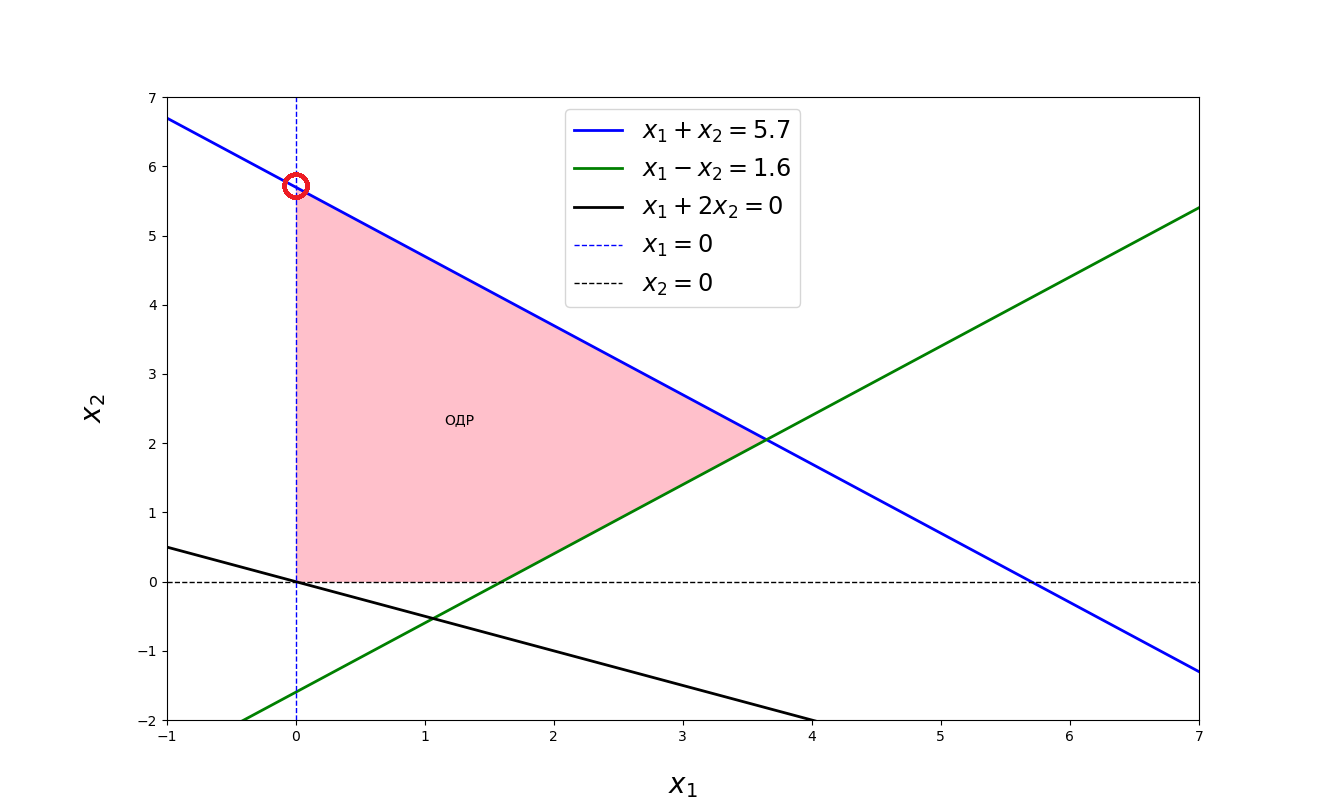
\includegraphics[width=1\textwidth]{graphic-solution}
	\caption{Графическое решение}
	\label{pic:graphic-solution}
\end{center}
\end{figure}

Только в точке $(0$, $5.7)$ достигается максимальное значение целевой функции, поэтому решение $x_1 = 0$, $x_2 = 5.7$ является единственным. 

\item Решим задачу методом полного перебора опорных точек.\\

Пусть $f(x_1, x_2) = x_1 + 2 x_2$, т.е $f$ -- целевая функция. Решив системы уравнений \ref{eq:2:2} -- \ref{eq:2:7}, найдём опорные точки:

\begin{equation}
\label{eq:2:2}
\begin{cases}
	x_1 = 0
	\\
	x_2 = 0
\end{cases}
\end{equation}

\begin{equation}
\begin{cases}
	x_1 = 0
	\\
	x_1 - x_2 = 1.6
\end{cases}
\Rightarrow
\begin{cases}
	x_1 = 0
	\\
	x_2 = -1.6
\end{cases}
\end{equation}

\begin{equation}
\begin{cases}
	x_1 - x_2 = 1.6
	\\
	x_2 = 0
\end{cases}
\Rightarrow
\begin{cases}
	x_1 = 1.6
	\\
	x_2 = 0
\end{cases}
\end{equation}

\begin{equation}
\begin{cases}
	x_1 + x_2 = 5.7
	\\
	x_2 = 0
\end{cases}
\Rightarrow
\begin{cases}
	x_1 = 5.7
	\\
	x_2 = 0
\end{cases}
\end{equation}

\begin{equation}
\begin{cases}
	x_1 - x_2 = 1.6
	\\
	x_1 + x_2 = 5.7
\end{cases}
\Rightarrow
\begin{cases}
	x_1 = 3.65
	\\
	x_2 = 2.05
\end{cases}
\end{equation}

\begin{equation}
\label{eq:2:7}
\begin{cases}
	x_1 = 0
	\\
	x_1 + x_2 = 5.7
\end{cases}
\Rightarrow
\begin{cases}
	x_1 = 0
	\\
	x_2 = 5.7
\end{cases}
\end{equation}

Теперь определим допустимость опорных точек и посчитаем значение целевой функции в них. Результаты приведены в таблице \ref{tab:target-function}.

\begin{table}[H]
\begin{center}
	\caption{Значения целевой функции в опорных точках}
	\label{tab:target-function}
	\def\tabcolsep{10pt}
	\def\arraystretch{1.23}
	\fontsize{13}{14}\selectfont
	\begin{tabular}{|c|c|c|}
		\hline 
		Опорная точка $(x_1,$ $x_2)$ & Принадлежит ОДР & Значение целевой функции \\ 
		\hline 
		$(0,$ $0)$ & + & 0 \\ 
		\hline 
		$(0,$ $-1.6)$ & -- & -3.2 \\ 
		\hline 
		$(1.6,$ $0)$ & + & 1.6 \\ 
		\hline 
		$(5.7,$ $0)$ & -- & 5.7 \\ 
		\hline 
		$(3.65,$ $2.05)$ & + & 7.75 \\ 
		\hline 
		$(0,$ $5.7)$ & + & 11.4 \\ 
	\hline 
	\end{tabular} 
\end{center}
\end{table}

По таблице \ref{tab:target-function} видно, что $x_1 = 0$, $x_2 = 5.7$ -- единственное решение.

\item Решим задачу симплекс-методом в матричной форме. Для этого приведём задачу к матричной форме:

\begin{equation}
\begin{aligned}
\begin{cases}
	max \left( c^T x \right)
	\\
	Ax = b
	\\
	b \geq 0
	\\
	x \geq 0
	\end{cases}
	%
	\text{, где }
	%
	A = \begin{pmatrix}
		1 & 1 & 1 & 0
		\\
		1 & -1 & 0 & 1
	\end{pmatrix},\\
	%
	x = \begin{pmatrix}
		x_1 \\ x_2 \\ x_3 \\ x_4
	\end{pmatrix} \text{, }
	%
	b = \begin{pmatrix}
		5.7 \\ 1.6
	\end{pmatrix} \text{, }
	%
	c = \begin{pmatrix}
		1 \\ 2 \\ 0 \\ 0
	\end{pmatrix}
\end{aligned}
\end{equation}

\begin{enumerate}

	\item Начальный базис $x_3$, $x_4$.\\
	 $x_1$, $x_2$ -- свободные переменные.
	
	\begin{displaymath}
		P = E = \begin{pmatrix}
			1 & 0 \\ 0 & 1
		\end{pmatrix}
	\end{displaymath}

	\item Текущий базис $x_3$, $x_4$\\
	\begin{displaymath}
		x^{\text{Б}} = P^{-1}b = \begin{pmatrix}
			1 & 0 \\ 0 & 1
		\end{pmatrix}
		\begin{pmatrix}
			5.7 \\ 1.6
		\end{pmatrix}
		=
		\begin{pmatrix}
			5.7 \\ 1.6
		\end{pmatrix}
	\end{displaymath}

	\item Допустимость базиса.
	
	$x^{\text{Б}} > 0 \Rightarrow$ базис допустимый.

	\item Оптимальность базиса.
	
	$c^\text{Б} = \begin{pmatrix}
		0 & 0
	\end{pmatrix}$

	$\forall j \notin \text{Б} : \Delta_j = c^\text{Б} P^{-1} A_j - c_j$

	$\Delta_1 = -1 < 0$, $\Delta_2 = -2 < 0 \Rightarrow$ базис неоптимальный.

	\item Вводимая в базис переменная.
	
	$k = argmin_j \Delta_j = 2$
	
	\item Выводимая из базиса переменная.
	
	$z = P^{-1} A_k = P^{-1} A_2 = \begin{pmatrix}
		1 & 0 \\ 0 & 1
	\end{pmatrix}
	\begin{pmatrix}
		1 \\ -1
	\end{pmatrix}
	=
	\begin{pmatrix}
		1 \\ -1
	\end{pmatrix}$
	
	$r = argmin_i\left\{ \frac{x_i^{\text{Б}}}{z_i} \Bigl|_{z_i > 0} \right\}$
	
	$\frac{x^{\text{Б}}}{z} = \begin{pmatrix}
		\frac{5.7}{1} \\ \frac{1.6}{-1}
	\end{pmatrix}
	=
	\begin{pmatrix}
		5.7 \\ -1.6
	\end{pmatrix}$
	
	$r = 3$

	\item Замена переменных.
	
	$x_r \leftrightarrow x_k$
	
	$x_3 \leftrightarrow x_2$
	
	\item Текущий базис $x_2$, $x_4$.
	
	\begin{displaymath}
		P = \begin{pmatrix}
			1 & 0 \\ -1 & 1
		\end{pmatrix}
	\end{displaymath}	
	
	\begin{displaymath}
		P^{-1} = \begin{pmatrix}
			1 & 0 \\ 1 & 1
		\end{pmatrix}
	\end{displaymath}		
	
	\begin{displaymath}
		x^{\text{Б}} = P^{-1}b = \begin{pmatrix}
			1 & 0 \\ 1 & 1
		\end{pmatrix}
		\begin{pmatrix}
			5.7 \\ 1.6
		\end{pmatrix}
		=
		\begin{pmatrix}
			5.7 \\ 7.3
		\end{pmatrix}
	\end{displaymath}
	
	\item Допустимость базиса.
	
	$x^{\text{Б}} > 0 \Rightarrow$ базис допустимый.
	
	\item Оптимальность базиса.
	
	$c^\text{Б} = \begin{pmatrix}
		2 & 0
	\end{pmatrix}$	
	
	$\Delta_1 = \begin{pmatrix}
		2 & 0
	\end{pmatrix}
	%
	\begin{pmatrix}
		1 & 0 \\ 1 & 1
	\end{pmatrix}
	%
	\begin{pmatrix}
		1 \\ 1
	\end{pmatrix}
	- 1 = 2 - 1 = 1 > 0
	$
	
	$\Delta_3 = \begin{pmatrix}
		2 & 0
	\end{pmatrix}
	%
	\begin{pmatrix}
		1 & 0 \\ 1 & 1
	\end{pmatrix}
	%
	\begin{pmatrix}
		1 \\ 0
	\end{pmatrix}
	- 0 = 2 - 0 = 2 > 0$	
	
	Базис $x_2$, $x_4$ оптимальный и решение $x_1 = 0$, $x_2 = 5.7$ единственное.		
	
\end{enumerate}

\item Решим задачу симплекс-методом в табличной форме.

По канонической форме (уравнение \ref{eq:2:1}) построим симплекс-таблицу \ref{tab:simplex:1}:

\begin{table}[H]
\begin{center}
	\caption{}
	\label{tab:simplex:1}
	\def\tabcolsep{18pt}
	\def\arraystretch{1.5}
	\fontsize{13}{14}\selectfont
	\begin{tabular}{|c|c||c||c|}
	\hline
	 & $x_1$ & $x_2$ & $b$ \\ 
	\hhline{|=|=|=|=|} 
	$x_3$ & -1 & \cellcolor{pink} -1 & 5.7 \\ 
	\hhline{|=|=|=|=|} 
	$x_4$ & -1 & 1 & 1.6 \\ 
	\hline 
	$f$ & 1 & 2 & 0 \\ 
	\hline 
	\end{tabular} 
\end{center}
\end{table}

\begin{displaymath}
\begin{cases}
	max_{j = 1, 2}(c_j) = 2
	\\
	min_{(c)}\left\{\frac{-b_i}{a_{ir}}\Bigl|_{a_{ir} < 0}\right\} = 5.7
\end{cases}
\Rightarrow
\text{разрезающий элемент равен } -1.
\end{displaymath}

Сделаем $x_2$ базисной переменной, а $x_3$ свободной. Разрезающий элемент заменим на 1. Элементы разрезающего столбца оставим без изменений. Элементы разрезающей строки умножим на -1. Оставшиеся элементы пересчитаем по правилу прямоугольника. Получим симплекс-таблицу \ref{tab:simplex:2}:

\begin{table}[H]
\begin{center}
	\caption{}
	\label{tab:simplex:2}
	\def\tabcolsep{18pt}
	\def\arraystretch{1.5}
	\fontsize{13}{14}\selectfont
	\begin{tabular}{|c|c||c||c|}
	\hline
	 & $x_1$ & $x_3$ & $b$ \\ 
	\hhline{|=|=|=|=|} 
	$x_2$ & 1 & \cellcolor{pink} 1 & -5.7 \\ 
	\hhline{|=|=|=|=|} 
	$x_4$ & 2 & 1 & -7.3 \\ 
	\hline 
	$f$ & 1 & 2 & -11.4 \\ 
	\hline 
	\end{tabular} 
\end{center}
\end{table}

Теперь разделим все элементы таблицы на разрезающий элемент (-1) и получим таблицу \ref{tab:simplex:3}:

\begin{table}[H]
\begin{center}
	\caption{}
	\label{tab:simplex:3}
	\def\tabcolsep{18pt}
	\def\arraystretch{1.5}
	\fontsize{13}{14}\selectfont
	\begin{tabular}{|c|c|c|c|}
	\hline
	 & $x_1$ & $x_3$ & $b$ \\ 
	\hline 
	$x_2$ & -1 & -1 & \cellcolor{green} 5.7 \\ 
	\hline
	$x_4$ & -2 & -1 & 7.3 \\ 
	\hline 
	$f$ & -1 & -2 & 11.4 \\ 
	\hline 
	\end{tabular} 
\end{center}
\end{table}

$\forall j \notin \text{\textbf{Б}}$, $c_j < 0$, поэтому $x_2$, $x_4$ оптимальный базис и решение $x_1 = 0$, $x_2 = 5.7$ единственное.

\item Введём дополнительное ограничение, отсекающее оптимальную точку: $x_2 \leq 5$.\\
Объединим это условие с системой \ref{eq:2:1} и приведем к канонической форме:

\begin{equation}
\label{eq:simpl:double:canonic}
\begin{cases}
	max \left( x_1 + 2 \cdot x_2 \right)
	\\
	x_3 = 5.7 - x_1 - x_2
	\\
	x_4 = 1.6 - x_1 + x_2
	\\
	x_5 = 5 - x_2
	\\
	x_1 \geq 0
	\\
	x_2 \geq 0
	\\
	x_3 \geq 0	
	\\
	x_4 \geq 0
	\\
	x_5 \geq 0
\end{cases}
\end{equation}	

Решим новую задачу двойственным симплекс-методом в табличной форме, в качестве начального базиса используя оптимальный базис исходной задачи --- $x_2$, $x_4$. В таблице \ref{tab:simplex:double:1} оптимальный базис исходной задачи.

\begin{table}[H]
\begin{center}
	\caption{}
	\label{tab:simplex:double:1}
	\def\tabcolsep{18pt}
	\def\arraystretch{1.5}
	\fontsize{13}{14}\selectfont
	\begin{tabular}{|c|c|c|c|}
	\hline
	 & $x_1$ & $x_3$ & $b$ \\ 
	\hline 
	$x_2$ & -1 & -1 & 5.7 \\ 
	\hline
	$x_4$ & -2 & -1 & 7.3 \\ 
	\hline 
	$f$ & -1 & -2 & 11.4 \\ 
	\hline 
	\end{tabular} 
\end{center}
\end{table}

Добавим новое условие

\begin{table}[H]
\begin{center}
	\caption{}
	\label{tab:simplex:double:2}
	\def\tabcolsep{18pt}
	\def\arraystretch{1.5}
	\fontsize{13}{14}\selectfont
	\begin{tabular}{|c||c||c|c|}
	\hline
	 & $x_1$ & $x_3$ & $b$ \\ 
	\hline 
	$x_2$ & -1 & -1 & 5.7 \\ 
	\hline
	$x_4$ & -2 & -1 & 7.3 \\ 
	\hhline{|=|=|=|=|}
	$x_5$ & \cellcolor{pink} 1 & 1 & -0.7 \\
	\hhline{|=|=|=|=|}
	$f$ & -1 & -2 & 11.4 \\ 
	\hline 
	\end{tabular} 
\end{center}
\end{table}

Псевдоплан $x_2$, $x_4$, $x_5$ допустимый, но не оптимальный. Разрезающий элемент выделен цветом.

Сделаем $x_1$ базисной переменной, а $x_5$ свободной. Разрезающий элемент заменим на 1. Элементы разрезающего столбца оставим без изменений. Элементы разрезающей строки умножим на -1. Оставшиеся элементы пересчитаем по правилу прямоугольника. Затем все элементы разделим на разрезающий. Получим симплекс-таблицу \ref{tab:simplex:double:3}:

\begin{table}[H]
\begin{center}
	\caption{}
	\label{tab:simplex:double:3}
	\def\tabcolsep{18pt}
	\def\arraystretch{1.5}
	\fontsize{13}{14}\selectfont
	\begin{tabular}{|c|c|c|c|}
	\hline
	 & $x_5$ & $x_3$ & $b$ \\ 
	\hline 
	$x_2$ & -1 & 0 & \cellcolor{green} 5 \\ 
	\hline
	$x_4$ & -2 & 1 & 5.9 \\ 
	\hline
	$x_1$ & 1 & -1 & \cellcolor{green} 0.7 \\
	\hline
	$f$ & -1 & -1 & 10.7 \\ 
	\hline 
	\end{tabular} 
\end{center}
\end{table}

Псевдоплан $x_1$, $x_2$, $x_4$ допустимый и оптимальный. Единственное решение $x_1 = 0.7$, $x_2 = 5$.

На рис. \ref{pic:additional-limit} представлено графическое решение новой задачи.

\begin{figure}[H]
\begin{center}
	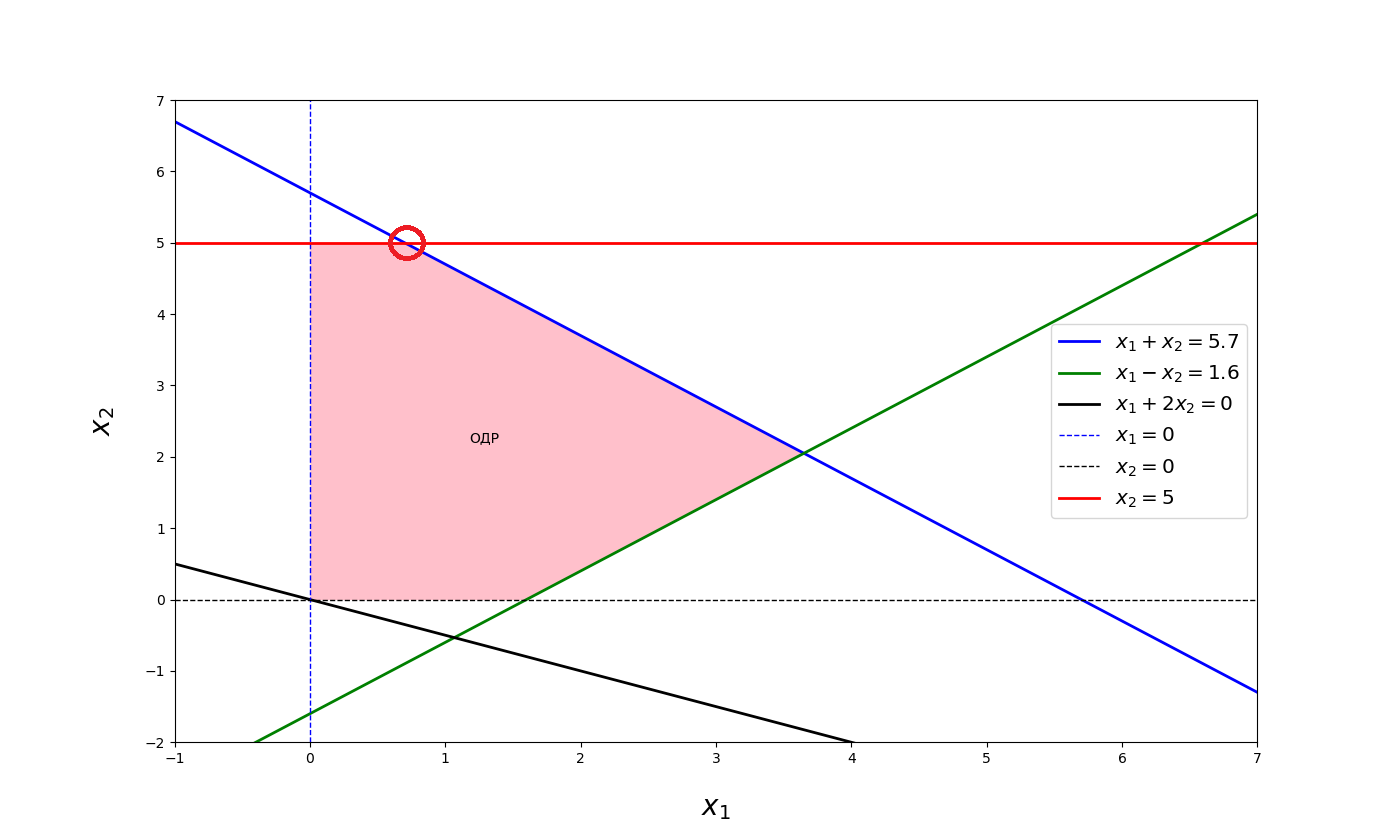
\includegraphics[width=1\textwidth]{additional-limit}
	\caption{Графическое решение}
	\label{pic:additional-limit}
\end{center}
\end{figure}

\item Сформулируем двойственную задачу по отношению к исходной:

\begin{displaymath}
\begin{cases}
	min \left( 5.7 \cdot y_1 + 1.6 \cdot y_2 \right)
	\\
	y_1 + y_2 \geq 1
	\\
	y_1 - y_2 \geq 2
	\\
	y_1 \geq 0
	\\
	y_2 \geq 0
\end{cases}
\end{displaymath}

\end{enumerate}

\end{document}